\section{Monte Carlo method}
In this section, we map the spin-boson model to the Ising model with long-range interactions on the imaginary axis by deriving the partition function of the spin-boson model in the imaginary time form.
And, we explain how to numerically calculate the response function $\mathrm{Im}[\chi(\omega)]$ by Monte Carlo method to the long-range Ising model.

First, we divide the spin-boson hamiltonian (\ref{hamiltonian}) into two parts:
\begin{eqnarray}
	H&=&\frac{\Delta\sigma_x}{2}+H_z,\\
	H_z&=&\sum_{\nu=L,R}\sum_k\omega_{\nu k } b_{\nu k}^{\dagger} b_{\nu k}+\sum_{\nu=L,R}\sum_k \frac{\sigma_z}{2}\lambda_{\nu k}(b_{\nu k}+b_{\nu k}^{\dagger}).
\end{eqnarray}
Then, the partition function $Z=\mathrm{Tr}[e^{-\beta H}]$ can be described as
 \begin{eqnarray}
	Z&=&Z_++Z_-,\\
	Z_{\pm}&=&\bra{\pm}\mathrm{Tr_{\mathrm{boson}}}[e^{-\beta H}]\ket{\pm},
\end{eqnarray}
where $\ket{\pm}$ means the eigen state of $\sigma_z$, i.e., $\sigma_z\ket{\pm}=\pm1\ket{\pm}$, 
and  $\mathrm{Tr_{\mathrm{boson}}}$ means the trace for the boson's degree of freedom.
Here, we introduce $\tilde{\sigma}_x(u)$ defined as  
$
\tilde{\sigma}_x(u)\equiv e^{iH_zu}\sigma_xe^{-iH_zu},
$
then we can expand $Z_+$ into
\begin{eqnarray}
	Z_+&=&\mathrm{Tr_{\mathrm{boson}}}\left[\bra{+}e^{-\beta H_z}e^{-\int_{0}^{\beta}du \Delta \tilde{\sigma}_{x}(u)/2}\ket{+}\right]\\
	&=&\sum_{n=0}^{\infty}\mathrm{Tr_{\mathrm{boson}}}
	\left[\bra{+}e^{-\beta H_z }\int_{0}^{\beta}d\tau_1 \ldots \int_{0}^{\tau_{2n-1}-\tau_c} d\tau_{2n}
	\left(\frac{\Delta}{2}\right)^{2n}\tilde{\sigma}_x(\tau_1) \ldots \tilde{\sigma}_x(\tau_{2n})\ket{+}\right].
\end{eqnarray}
where $\tau_c$ is the cutoff on the imaginary time axis and it is given by $\tau_c=1/\omega_c$.
By calculating the trace for the boson's degree of freedom, we can derive the instanton-like partition function with n-kink pairs? \cite{Leggett87,Volker98}:
\begin{eqnarray}
	Z_+&=&Z_0\sum_{n=0}^{\infty}\left(\frac{\Delta\tau_c}{2}\right)^{2n}\int_{0}^{\beta}\frac{d\tau_1}{\tau_c} \ldots \int_{0}^{\tau_{2n-1}-\tau_c} \frac{d\tau_{2n}}{\tau_c}
	\mathrm{exp}\left[\sum_{j>i}^{2n}(-1)^{i+j}W(\tau_j-\tau_i)\right],
	\label{z_+}
\end{eqnarray}
where $Z _0$ is the partition function of  bosons in the heat bath,
and  $W(\tau)$ is given by 
\begin{eqnarray}
	W(\tau)&=&\int_{0}^{\infty}d\omega \frac{I(\omega)}{\omega^2}
	\frac{\mathrm{cosh}(\beta\omega/2)-\mathrm{cosh}(\beta\omega/2-\tau)}{\mathrm{sinh}(\beta\omega/2)}.
	\label{kink_interaction}
\end{eqnarray}
%付録?
We can calculate  $Z_{-}$ in the same way.
%
If we regard $\tilde{\sigma}_x(\tau_{j})$ as a kink charge, 
Eq. ($\ref{z_+}$) can be regarded as the ``kink'' representation of the one-dimensional Ising model with the  system states distinguished by the kink-degree of freedom $\{ \tilde{\sigma}_x(\tau_i)\}$.
Now, we consider rewriting it to the ``spin'' representation.
Generally, the partition function of  the one-dimensional Ising model with long-range interactions with the lattice constant $a$ 
is written in the kink representation as 
\begin{eqnarray}
	Z_{\mathrm{ising}}&=&\sum_{n=0}^{\infty}y^{2n}\int_{0}^{\beta}\frac{d\tau_1}{a} \ldots \int_{0}^{\tau_{2n-1}-a} \frac{d\tau_{2n}}{a}
	\mathrm{exp}\left[\sum_{j>i}^{2n}(-1)^{i+j}4U\left(\frac{\tau_j-\tau_i}{a}\right)\right],
	\label{Z_ising_kink}
\end{eqnarray}
where $U(\tau)$ is the kink-kink interaction, and $y$ is the chemical potential which satisfies $y=e^{2U(0)}$.
According to \cite{Volker98,Cardy81}, we can calculate the spin-spin interaction $V(n)$ from the kink-kink interaction $U(n)$ by the following recurrence relation:
\begin{eqnarray}
	V(n)=U(n+1)-2U(n)+U(n-1),\ (n:\mathrm{integer}>0),
	\label{V}
\end{eqnarray}
then, Eq. (\ref{Z_ising_kink}) is described by $V(n)$ as 
\begin{eqnarray}
	Z_{\mathrm{ising}}=\sum_{S_1 \ldots S_N}\mathrm{exp}\left[-\sum_{j>i}V(j-i)S_iS_j\right],
	\label{Z_ising_spin}
\end{eqnarray}
where $S_i,(i:\mathrm{integer})$ is the spin of the $i$th site, $N$ is the total number of sites, and $S_{i}$
satisfies the boundary condition $S_{i}=S_{i+N}$ (Fig. \ref{fig:ising_model}).
\begin{figure}[tb]
	\centering
	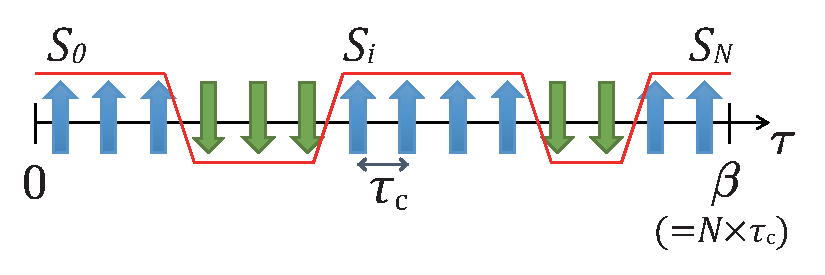
\includegraphics[height=4.0cm]{ising_model.eps}
	\caption{
	 the one-dimensional Ising model with long-range interactions on the imaginary $\tau$-axis.
	}
	\label{fig:ising_model}
\end{figure}
In this study, we divide $\beta$ in length on the $\tau$-axis into $N$ parts,
i.e., $\tau_c=\beta/N$.
Then, we put Ising spins on the each sites and chose $V(n)$ as Eq. (\ref{Z_ising_kink}) becomes our desiring partition function(\ref{z_+}).
Specifically, we decide $U(n)$ from $W(\tau)$, and calculate $V(n)$ by Eq. (\ref{V}).
Actually, we can derive $V(n)\propto n^{-(s+1)}$ for the large enough total number of sites $N$, i.e., $n/N\ll1$. 
In this way, we can map the spin-boson model to  the one-dimensional Ising model with long-range interactions.

Now, we remark the algebraic relation between the response function $\chi( \omega)$ and the spin-correlation function $C(\tau)$:
\begin{eqnarray}
	\chi(\omega)&=C(i\omega_n\rightarrow\omega+i\delta),\\
	\label{pade}
	C(i\omega_n)&=\int_{0}^{\beta}d\tau e^{i\omega_n \tau}C(\tau),\\
	\label{fourier}
	C(\tau)&=\average{\sigma_z(\tau)\sigma_z(0)},
\end{eqnarray}
where Eq. (\ref{pade}) means the analytic continuation.
These relations means we can derive $\mathrm{Im}[\chi( \omega)]$ by calculating $C(\tau)$.
And, we can derive $C(\tau)$ by calculating the spin correlation $\average{S_i S_0}$ of the long-range Ising model because they satisfies
$
\average{\sigma_z(\tau_i)\sigma_z(0)}\simeq \average{S_i S_0}.
$
%
In this study, we use the Monte Carlo method to calculate $C(\tau)$ of the Ising model derived from Eq. (\ref{Z_ising_spin}). But, it takes very long time to numerically calculate $C(\tau)$ because the Ising model derived from Eq. (\ref{Z_ising_spin}) has $r^{-(s+1)}$ long-range interactions. Especially, this problem notably appears in the low temperature. It is known that if you use the single flip method \cite{MetropolisMethod}, the relaxation time of the system diverges near the critical temperature (called ``critical slowing down''). 
This problem can be solved by the cluster-flip method like the Wolff algorithm\cite{Wolff89}.
In this study, we use an efficient Monte Carlo method based on the Wolff algorithm developed by E.Luijten \cite{Luijten95}.
The Luijten's algorithm utilizes the cumulative frequency distribution and in this algorithm we need not look at all spins in order to build a cluster but calculate the site at which the spin to add into a cluster first appears. 
Actually, we can realize more efficient implementation by making use of the bisection method to calculate the site.
In this way, we adopt the Wolff method utilizing the cumulative frequency distribution to calculate the spin correlation $\average{S_i S_0}$.

